\chapter{Estudo de Caso}
\label{est}
\section{Software Público Brasileiro}
\label{est:sof}

O portal do Software Público Brasileiro (SPB) é um espaço virtual, criado em 12 de 
abril de 2007, que agrega um conjunto de softwares desenvolvidos nas áreas de saúde, 
educação, saneamento, gestão de TI, TV Digital e Geoprocessamento. Os serviços do
SPB são acessados não só no Brasil, mas também por outros países como por exemplo:
Uruguai, Argentina, Portugal, Venezuela, Chile e Paraguai. A politica de compartilhamento
de software resulta em uma gestão de recursos e gastos de informática mais racionalizada,
ampliação de parcerias e reforço da politica de software livre no setor público~\cite{spb}.

O novo Portal do Software Público Brasileiro é composto de:

\begin{itemize}
    \item Lista de discussão (Mailman).
    \item Plataforma de redes sociais com blog, e-Portifólios, RSS, discussão 
    temática, agenda de eventos, galeria de imagens, e demais funcionalidades de um CMS (Noosfero).
    \item Sistema de controle de versão, repositório de código-fonte e ambiente 
    desenvolvimento colaborativo (GitLab).
    \item Autenticação única, busca e integração de ferramentas a fim de tornar 
    a navegação intuitiva e transparente entre as diversas ferramentas que compõem 
    o novo Portal (Colab).
\end{itemize}

\subsection{Metodologia de Desenvolvimento}
\label{est:sof:met}

O Software Público Brasileiro foi desenvolvido com base no Scrum. O
Scrum é um framework para o desenvolvimento e manutenção de produtos usado desde
o incio dos anos 90 que possui a característica de permitir que vários processos
e tecnicas possam ser empregadas juntamente a ele. Os três valores essenciais do
Scrum são:

\begin{itemize}
    \item Leveza.
    \item Simples de entender.
    \item Difícil de dominar.
\end{itemize}

O Scrum é fundamentado nas teorias empíricas de controle de processo, ou seja,
utiliza o conhecimento vindo de experiencias e das decisões passadas. Por isto, este 
framework emprega uma abordagem iterativa e incremental para permitir aperfeiçoar
a previsibilidade e os riscos. No Scrum, cada componente é essencial
para o sucesso, por isso existem regras especificas para os times, artefatos e
papéis dentro do framework.


\subsubsection{Práticas do Scrum}
\label{est:sof:met:pra}

O Scrum define algumas práticas que são aplicadas durante o desenvolvimento com 
o objetivo de minimizar a necessidade de reuniões. Estas práticas podem ser eventos
com uma duração definida e buscam aumentar as interações entre as pessoas. A lista
abaixo apresenta esses eventos e suas respectivas descrições.

\begin{itemize}
    \item \textbf{Sprint:} Um intervalo de tempo em que são desenvolvidos os itens
        propostos. Este intervalo geralmente é de duas a quatro semanas e ao final
        de cada sprint, um incremento de software é entregue.
    \item \textbf{Sprint Review:} Ao final de cada sprint o time revisa as atividades
        realizadas durante o período em que a sprint ocorreu. São levantados pontos de
        melhoria e quais foram os pontos fortes do time.
    \item \textbf{Sprint Planning:} No inicio de cada sprint, é feita uma reunião em
        que são priorizadas as atividades que serão realizadas.
    \item \textbf{Product Backlog:} Conjunto de itens que serão desenvolvidos no projeto.
        A cada sprint um conjunto de itens são escolhidos, retirados do \textit{Product
        Backlog} e implementados.
\end{itemize}

\subsection{Organização do Trabalho}
\label{est:sof:org}

O Software Público Brasileiro utiliza o Scrum juntamente com o XP e metodologias
ágeis para o seu desenvolvimento. Sendo assim, o projeto é dividido em dois níveis,
o nível operacional e um nível estratégico. Dentro do nível estratégico são definidas
as metas estratégicas de cada \textit{release}, o período de duração, e as épicas
de negocio. A medida que desce-se o nível a partir das metas estratégicas e nos
aproximamos do nível operacional, o grau de granularidade aumenta até chegar a
micro atividades. Podemos ver essa divisão ocorrendo nas figuras~\ref{fig:epics-diagram} 
e~\ref{fig:epics-wiki} abaixo, que mostram como essa quebra é feita e como isso acontece 
na Wiki do projeto.

\newpage
\begin{figure}[h]
    \centering
        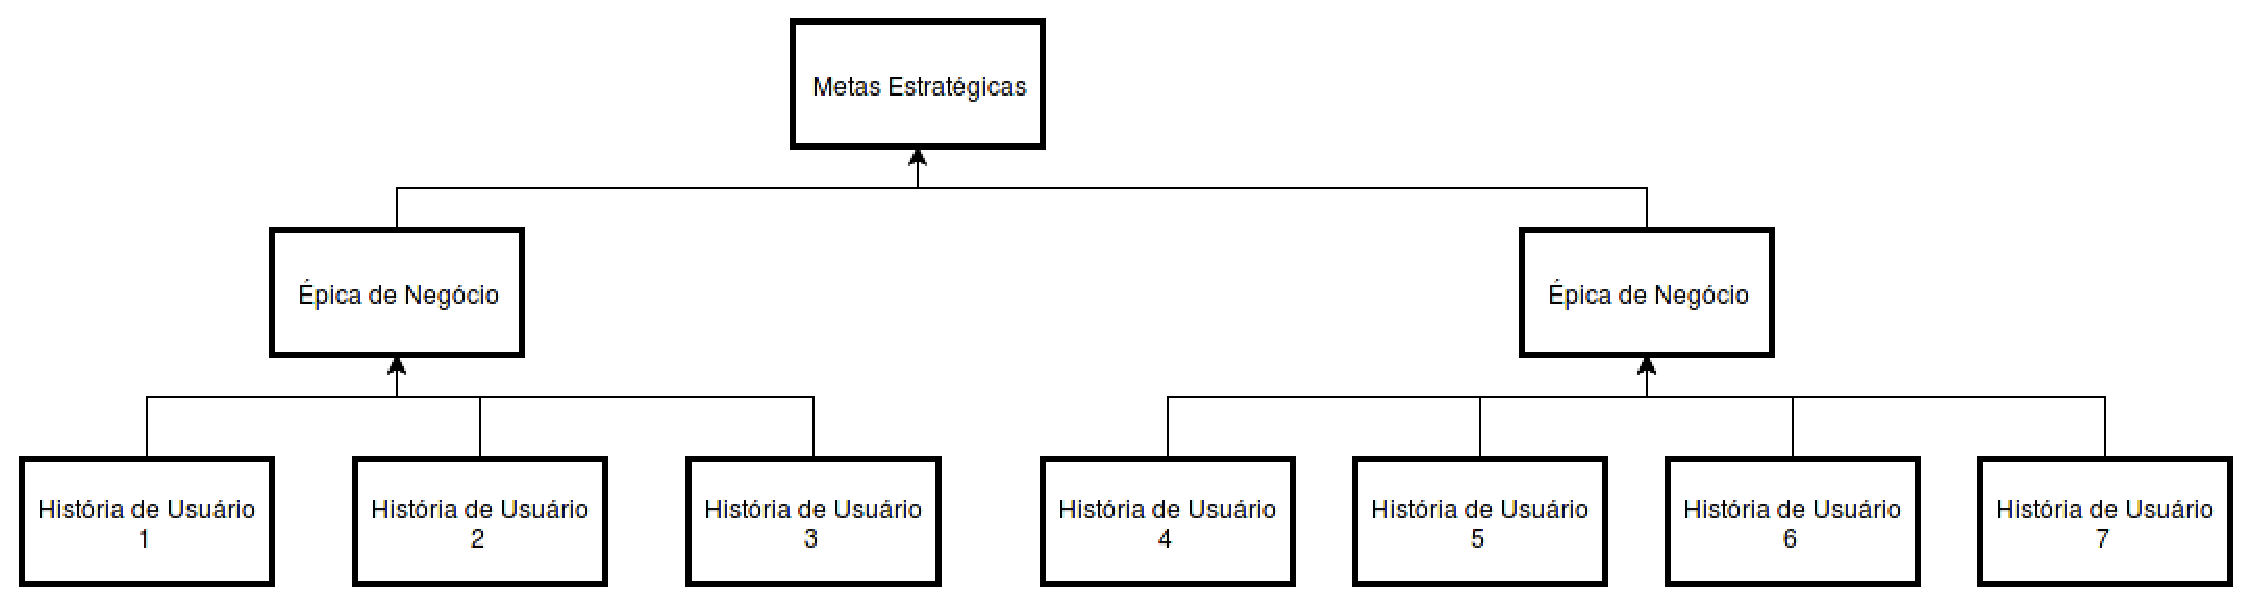
\includegraphics[keepaspectratio=true,scale=0.3]{figuras/epics-diagram.eps}
    \caption{Diagrama de Metas Estratégicas e Épicas de Negócio no SPB}
    \label{fig:epics-diagram}
\end{figure}

\begin{figure}[h]
    \centering
        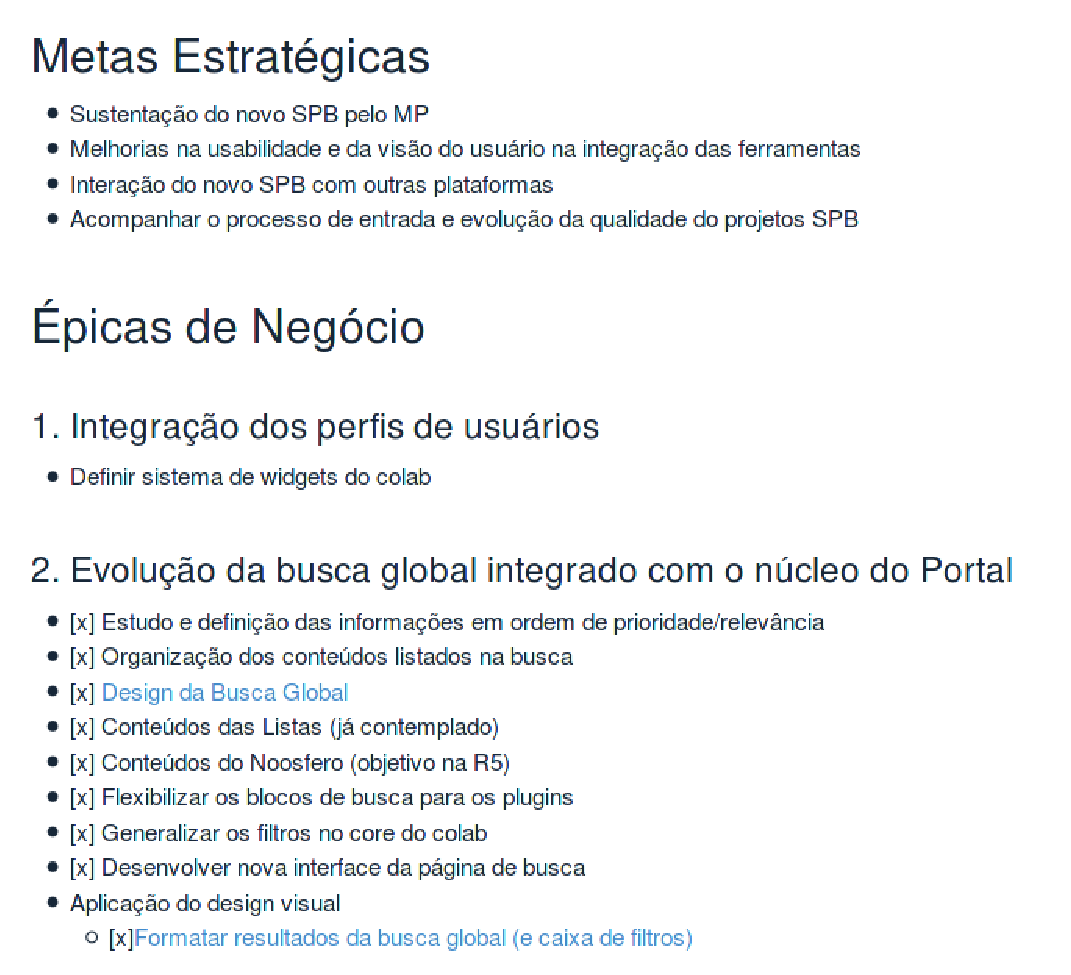
\includegraphics[keepaspectratio=true,scale=0.5]{figuras/wiki.eps}
    \caption{Wiki do SPB com as Métas de Estratégicas e Épicas de Negócio}
    \label{fig:epics-wiki}
\end{figure}

Já dentro do nível operacional existem as histórias de usuário e as atividades.
Dentro do SPB, as histórias de usuário são tratadas como \textit{milestones} 
e as atividades como \textit{issues} do Gitlab. Dentro de uma \textit{sprint}
cada time escolhe uma ou mais  histórias, do backlog da release, e realiza a divisão
de suas atividades entre seus membros. A utilização da ferramenta Gitlab permite
que as atividades possam ser comentadas e acompanhadas pelos usuários, facilitando,
desta forma, o acompanhamento do projeto tanto por parte do Ministério do Planejamento
Orçamento e Gestão e dos desenvolvedores. As imagens~\ref{fig:milestone} e~\ref{fig:issue}
abaixo mostram a estrutura de uma história e de uma atividade.

\newpage
\begin{figure}[h]
    \centering
        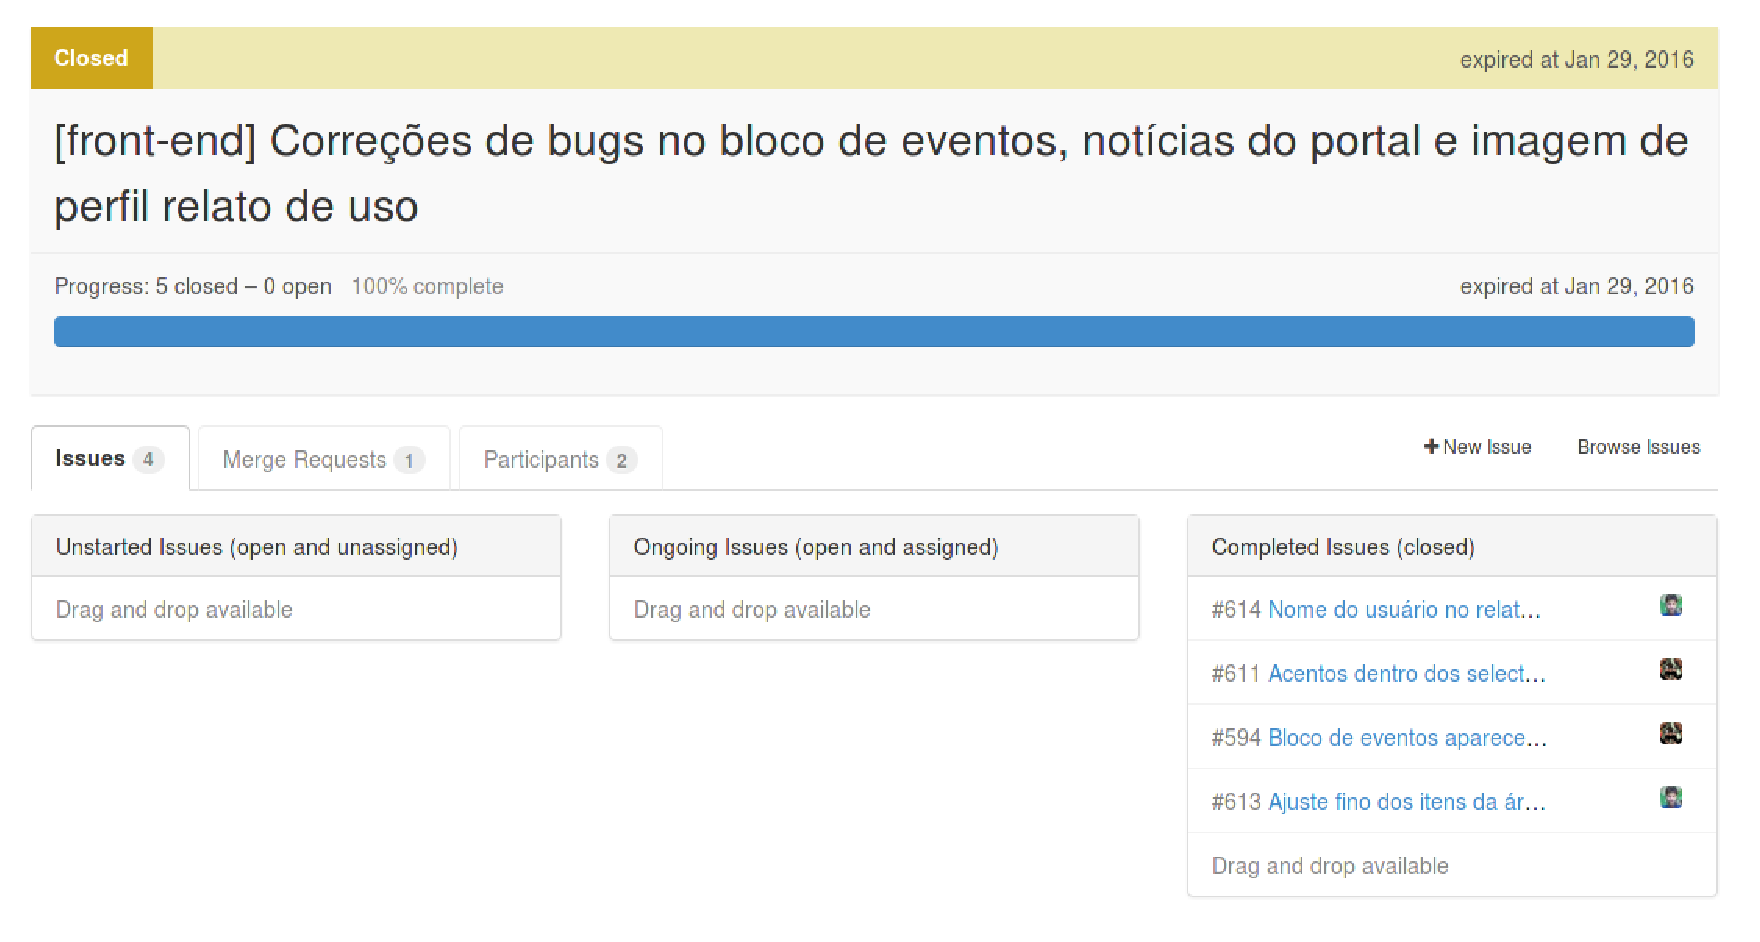
\includegraphics[keepaspectratio=true,scale=0.5]{figuras/milestone.eps}
    \caption{Estrutura de um Milestone no SPB}
    \label{fig:milestone}
\end{figure}


\begin{figure}[h]
    \centering
        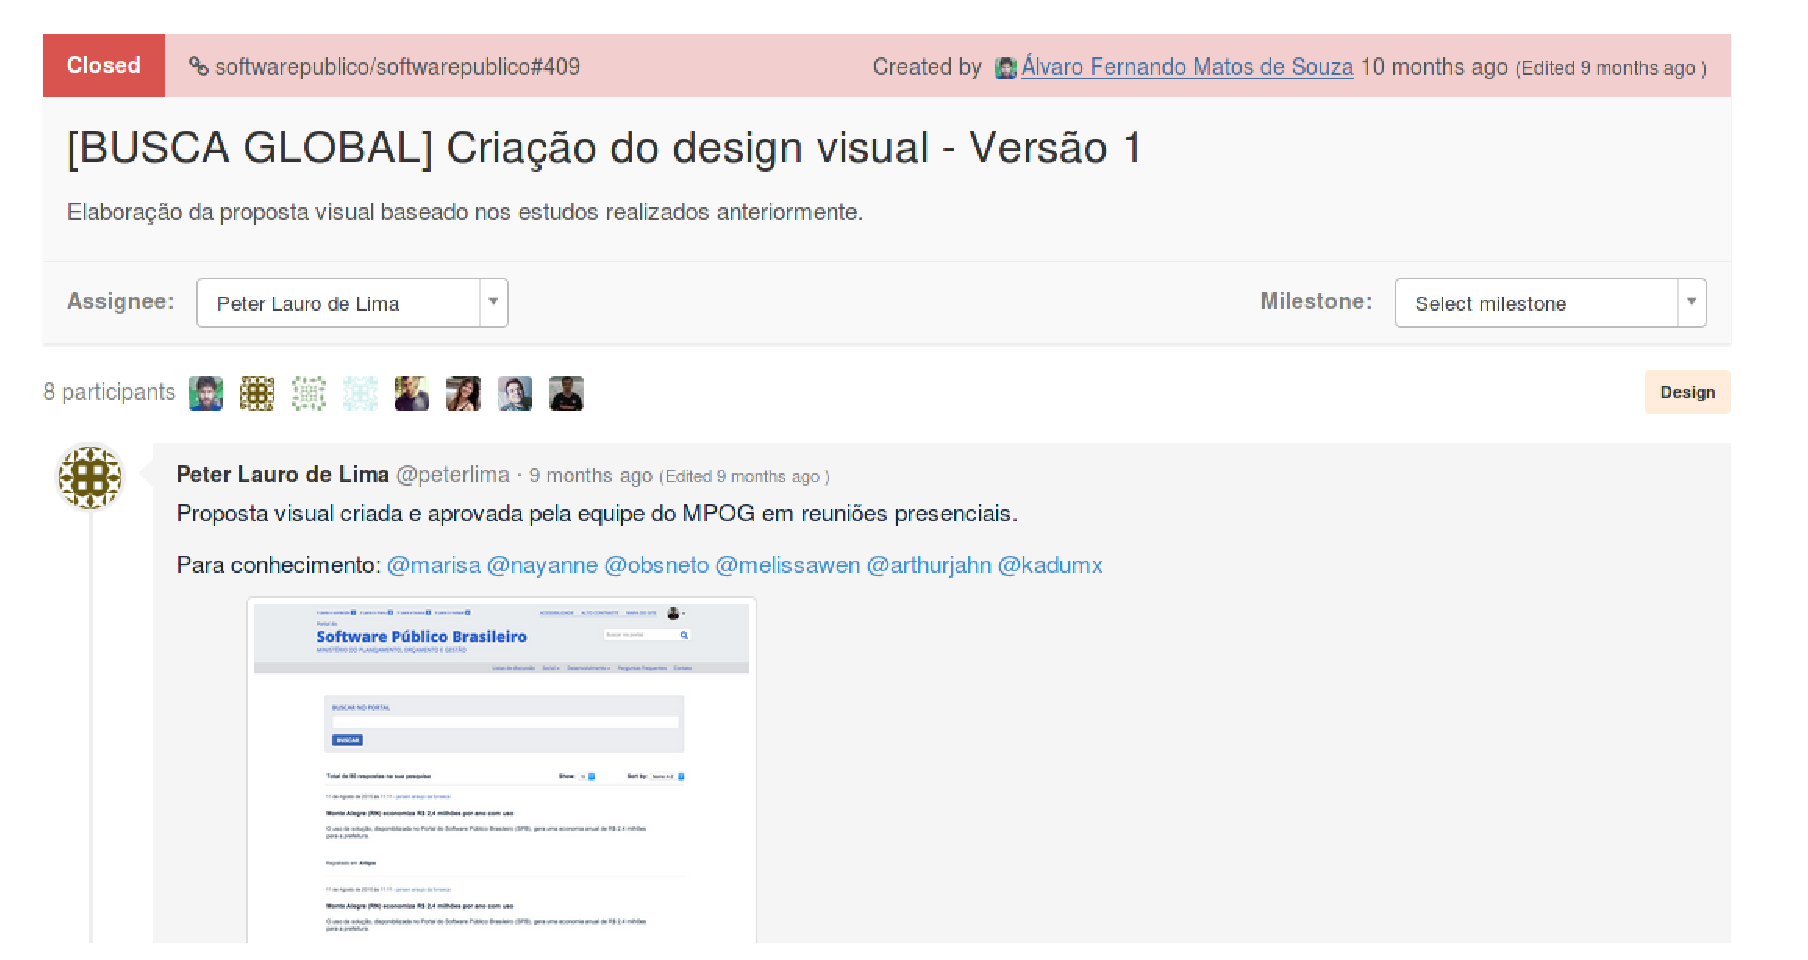
\includegraphics[keepaspectratio=true,scale=0.5]{figuras/issue.eps}
    \caption{Estrutura de uma Issue no SPB}
    \label{fig:issue}
\end{figure}

A escolha do SPB como um caso piloto foi estratégica, visto que é um projeto de 
domínio público e utilizando o Gitlab, é possível exportar informações de
desenvolvedores, atividades, histórias e épicas, além disto é possível extrair
informações especificas relacionadas ao código fonte do projeto. Sem este tipo
de acesso a informação seria praticamente impossível a execução deste experimento.
Outro fator determinante é a forma com o que o SPB concentra o planejamento de release
dentro da repositório, o permite com que a relação entre as atividades seja evidenciada
mais facilmente.

\section{Ranqueamento de Páginas no SPB}
\label{est:ran}

Essa sessão apresenta como o algoritmo de ranqueamento de páginas foi aplicado
ao Software Público Brasileiro de forma a extrair a relevância das \textit{issues}.
Como foi dita na sessão~\ref{est:sof:org}, a escolha deste projeto para o estudo de caso
foi estratégica de forma a facilitar a execução deste experimento, já que o SPB possui 
estrutura e condições favoráveis a isso.

\subsection{Vértices e Arestas}
\label{est:ran:ver}

Como foi visto na sessão~\ref{ref:ran} a utilização do algoritmo de ranqueamento
de páginas depende que inicialmente exista um grafo direcionado.\footnote{Um grafo direcionado, 
ou dígrafo, $D$ consiste de um conjunto finito de elementos não vazios $V(D)$
chamados de vértices e um conjunto finito $A(D)$ de pares ordenados de vértices
distintos chamados arcos. Desta forma, $V(D)$ é chamado de conjunto de vértices e
$A(D)$ o conjunto de arcos de $D$~\cite{bang}.}

Para que um grafo do SPB fosse gerado, foi utilizada a API do Gitlab juntamente
com um \textit{script Python} para que todas as \textit{issues}, \textit{milestones} e
comentários fosse exportado em formato JSON. Como foi dito, o algoritmo de
ranqueamento de páginas precisa de um dígrafo para ser executado, uma das adaptações
deste \textit{script} é que em alguns casos os grafos gerados não eram direcionados,
e por isto, estes grafos tiveram que ser convertidos em grafos direcionados substituindo
cada um dos arcos ou arestas por um arco de entrada e um de saída, este processo pode
ser visto nas figuras~\ref{fig:undirected} e~\ref{fig:directed}.

\begin{figure}[h]
    \centering
        
\includegraphics[keepaspectratio=true,scale=0.5]{figuras/undirected.eps}
    \caption{Issues antes da conversão dos arcos}
    \label{fig:undirected}
\end{figure}

\begin{figure}[h]
    \centering
        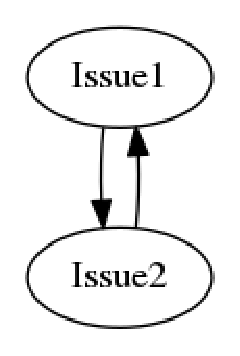
\includegraphics[keepaspectratio=true,scale=0.5]{figuras/directed.eps}
    \caption{Issues depois da conversão dos arcos}
    \label{fig:directed}
\end{figure}

\newpage
\subsubsection{Issues}
\label{est:ran:iss}

Como o foco do estudo é analisar a relevância das \textit{issues}, o dígrafo 
foi gerado com base nelas. Dentro do grafo, cada \textit{issue} foi tratada
como um vértice, e as arestas eram formadas a medida que uma \textit{issue}
era marcada, através de comentários ou eventos, dentro de outra. A figura
~\ref{fig:issue-comment} exemplifica esse processo.

\begin{figure}[h]
    \centering
        
\includegraphics[keepaspectratio=true,scale=0.5]{figuras/issue-comment.eps}
    \caption{Exemplo de comentário com marcação de issue}
    \label{fig:issue-comment}
\end{figure}

Para a realização deste processo foram analisados os comentários de todas as 879
\textit{issues} no repositório do SPB. O dígrafo gerado por esse processo, foi
então utilizado para a aplicação do algoritmo de ranqueamento de páginas, a figura
~\ref{fig:issue-graph} demonstra como esse grafo se apresenta.

\begin{figure}[h]
    \centering
        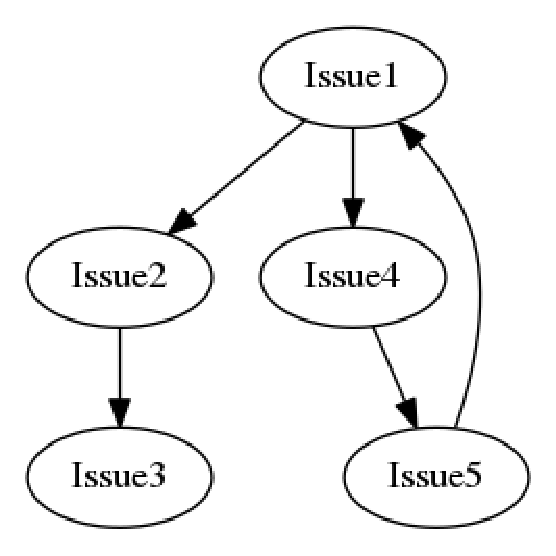
\includegraphics[keepaspectratio=true,scale=0.5]{figuras/issue-graph.eps}
    \caption{Demonstração de grafo das issues}
    \label{fig:issue-graph}
\end{figure}


\subsubsection{Milestones}
\label{est:ran:mil}

Dentro do projeto SPB, um \textit{milestone} é uma história com um conjunto de 
\textit{issues} associadas. Para que fosse possível uma maior aproximação com
o ranqueamento de páginas considerou-se que todas as \textit{issues} dentro de
um \textit{milestones} estão interligadas, de forma que elas formem um grafo completo,
essa abstração pode ser vista na figura~\ref{fig:milestone-graph}.
\footnote{Um grafo $G$ é considerado como completo se cada par de vértices distintos em $G$
são adjacentes~\cite{bang}.}

\newpage
\begin{figure}[h]
    \centering
        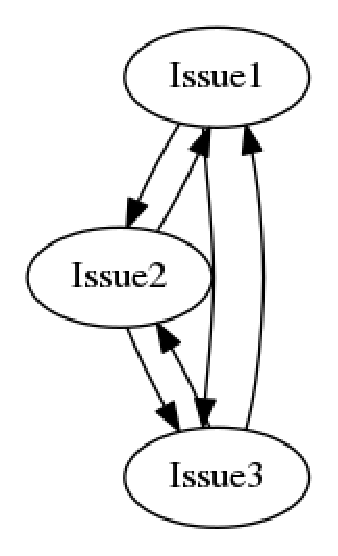
\includegraphics[keepaspectratio=true,scale=0.5]{figuras/milestone-graph.eps}
    \caption{Demonstração de grafo das issues em um mesmo  milestones}
    \label{fig:milestone-graph}
\end{figure}

\section{Resultados}
\label{est:res}

Utilizando-se das abstrações descritas na seção \ref{est:ran} foi possível gerar um grafo representando as \textit{issues} do SPB. Este grafo apresenta as \textit{issues} mais altamente conectadas no centro e as menos conectadas nas bordas. Na figura \ref{fig:graph}, é possível perceber que a grande maioria das \textit{issues} tem poucas conexões, ou seja, possuem poucos comentários de marcação, além disto, em alguns casos estas \textit{issues} não estavam associadas a nenhum \textit{milestone}. Esse comportamento pode denotar um baixo índice de comunicação entre a equipe de desenvolvimento e os \textit{stakeholders} no inicio do projeto.

\begin{figure}[h]
    \centering
        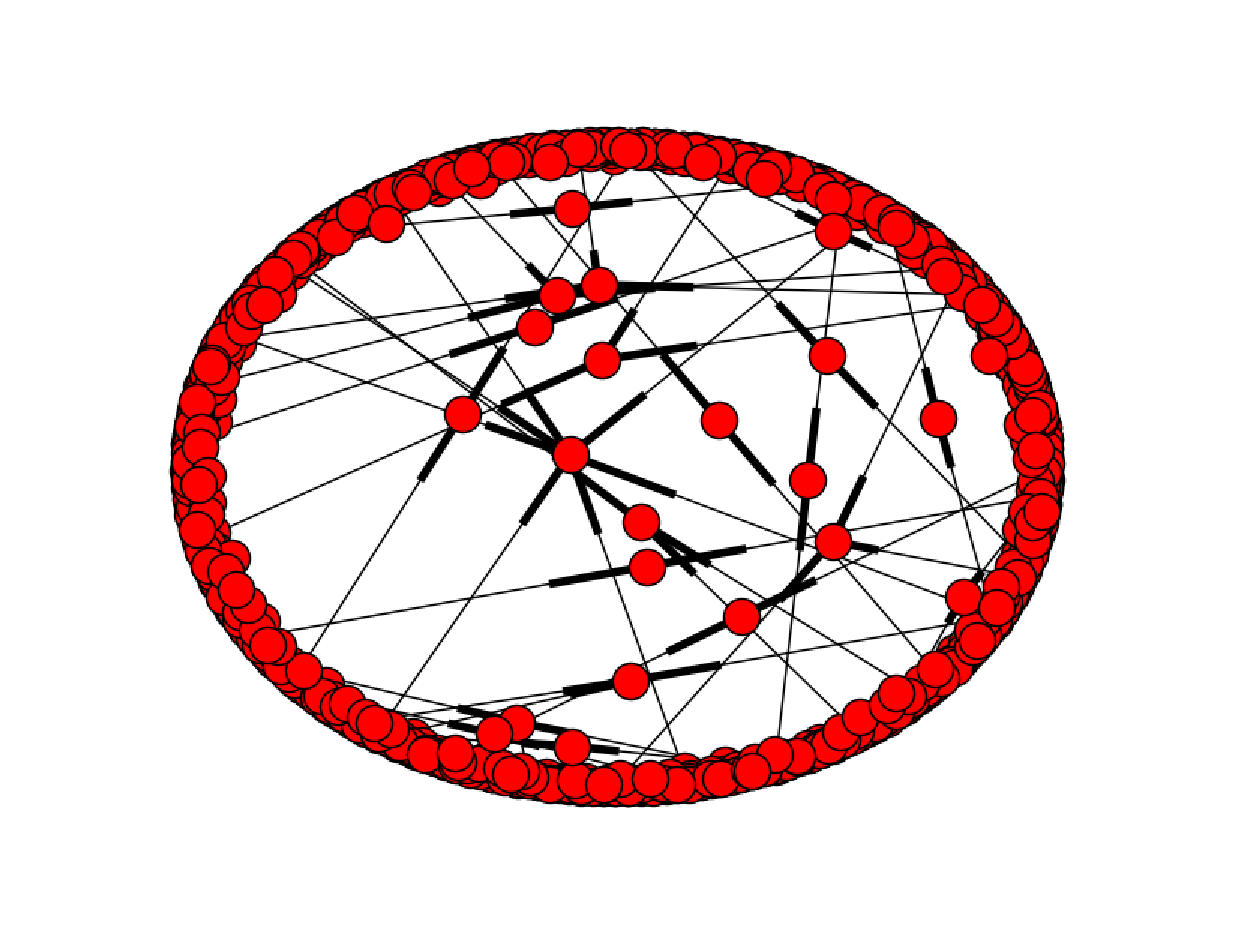
\includegraphics[keepaspectratio=true,scale=0.5]{figuras/graph.eps}
    \caption{Grafo das issues do SPB}
    \label{fig:graph}
\end{figure}

A partir do grafo representado na figura \ref{fig:graph}, foi executado o algoritmo de ranqueamento de páginas, o algoritmo utilizado foi o \textit{Page Ranking}, discutido na seção \ref{ref:ran}. Para permitir a execução do algoritmo, foram utilizadas as abstrações para \textit{issues} e \textit{milestones} discutidas nas seções \ref{est:ran:iss} e \ref{est:ran:mil}. Após a execução, o algoritmo exporta as \textit{issues} associadas a um valor numérico, de forma que, quanto maior o valor associado a uma \textit{issue}, maior o seu ranque relativo. No SPB, as dez \textit{issues} com o maior ranque relativo estão apresentadas na tabela \ref{tab:pagerank}. 

\begin{table}[h]
        \centering
	\label{tab:pagerank}
	
        \begin{tabular}{| >{\centering}m{10cm} | c |}
        	\toprule
		\textbf{Issue} & \textbf{Pagerank} \\
		\midrule
		Moderação do valor dos recursos economizados do relato de uso & 0.0059332219490603475 \\ \hline
                Configurar o NGINX para servir os dados do syslog & 0.003453026773943251 \\ \hline
                Exibir mensagem de erro próxima ao campo instituição no relato de uso &  0.003453026773943251 \\\hline
                Subir o gitlab 8.5 usando o pacote feito. & 0.003453026773943251 \\\hline
                Melhora da busca global & 0.003453026773943251 \\\hline
                Tela branca em Editar blocos laterais de comunidade & 0.003453026773943251 \\\hline
                Importar as notícias wiki do portal &  0.0030396609114237347 \\\hline
                Cadastro de usuário quebrado (username: boscojr) & 0.002626295048904218 \\\hline
                Adicionar email do usuário na Tela de processar solicitação de Entrar na comunidade. & 0.002626295048904218 \\\hline
                Retirar pergunta por SISP na criação de uma nova instituição? & 0.002626295048904218 \\\hline
		\bottomrule      
 	\end{tabular}
\end{table}

Com base nas \textit{issues} melhores ranqueadas, foi possível perceber que alguns termos aparecem com maior frequência, são eles: \textbf{Relato de Uso}, \textbf{Busca Global}, \textbf{Gitlab} e \textit{SISP}. Outras das \textit{issues} que aparecem com o ranque alto, estão ligadas a atividades de manutenção, sejam elas: correção de \textit{bugs}, melhorias de \textit{front-end} e infraestrutura. Desta forma, aparentemente, as \textit{features} de implementação do relato de uso, da busca global, atualização do Gitlab e algumas das correções de \textit{bugs} foram consideradas de maior importância do que aquelas que apresentaram grau de relevância menor. Apesar de ter sido possível relacionar a relevância das \textit{issues} e as \textit{features} do SPB, este processo foi feito manualmente e não foi automatizado para esta primeira metade do trabalho, um ponto que deve ser atacado na próxima parte.
